\documentclass[12pt,a4paper]{report}
\usepackage[utf8]{inputenc}
\usepackage[T1]{fontenc}
\usepackage{lmodern}
\usepackage{amsmath}
%\usepackage{algorithm}
\usepackage{listings}
%\usepackage{standalone}
%\usepackage{algpseudocode}
\usepackage[linesnumbered,lined,boxed,commentsnumbered]{algorithm2e}
\newcommand\mycommfont[1]{\footnotesize\ttfamily{#1}}
\SetCommentSty{mycommfont}
\usepackage{verbatim}
\usepackage{tabularx}
%\usepackage{program}
%\input{externaldoc}
%\input{verticalblock}
%\algrenewcommand\algorithmicindent{1.0em}
\usepackage{minitoc}
\usepackage{float}
\usepackage{hyperref}
\usepackage{physics}
\usepackage{color}
\usepackage{subfiles}
\usepackage{pdfpages}
\usepackage[ED=SDM-PMat, Ets=UT3]{tlsflyleaf}

\hypersetup{
 colorlinks=true,
 linkcolor=blue,
 filecolor=blue,
 urlcolor=blue,
 citecolor=blue
}
\usepackage{mathpazo,libertine}



\newcommand{\alert}[1]{\textcolor{red}{#1}}
\newcommand{\Hij}[3][\hat{H}]{\mel{#2}{#1}{#3}}
%\newcommand{\ket}[1]{| #1 \rangle}

%sizes
\newcommand{\Ndet}{{N_\text{det}}}
\newcommand{\Ngen}{{N_\text{gen}}}
\newcommand{\Nsel}{{N_\text{sel}}}
\newcommand{\Norb}{{N_\text{orb}}}
\newcommand{\Nelec}{{N_\text{elec}}}
\newcommand{\Nalpha}{{N_\text{elec}^\alpha}}
\newcommand{\Nbeta}{{N_\text{elec}^\beta}}
\newcommand{\Nint}{{N_\text{int}}}
\newcommand{\Nst}{{N_\text{states}}}
\newcommand{\Ndav}{{N_\text{dav}}}
\newcommand{\Nperm}{{N_\text{perm}}}
\newcommand{\Na}{{N_\alpha}}
\newcommand{\Nb}{{N_\beta}}
\newcommand{\Ne}{{N_\text{elec}}}
\newcommand{\NFCI}{N_\text{FCI}}

%bitmasks
\newcommand{\bit}[1]{{\texttt{#1}}}
\newcommand{\bitI}{{\texttt{I}}}
\newcommand{\bitP}{{\texttt{P}}}
\newcommand{\bitJ}{{\bit{J}}}
\newcommand{\bitK}{{\bit{K}}}
\newcommand{\bitx}[2]{{\texttt{#1}_{#2}}}
\newcommand{\bitIsigma}{{\bitx{I}{\sigma}}}
\newcommand{\bitPsigma}{{\bitx{P}{\sigma}}}
\newcommand{\binary}[1]{{#1_{\mathtt{2}}}}
\newcommand{\TRUE}{{\text{\texttt{TRUE}}}}
\newcommand{\FALSE}{{\text{\texttt{FALSE}}}}


%acronyms
\newcommand{\HF}{{\text{HF}}}
\newcommand{\QP}{{ \textsc{Quantum Package} }}

%energies
\newcommand{\EDMC}{E_\text{DMC}}
\newcommand{\EPT}{E_\text{PT2}}
\newcommand{\Ecor}{E_\text{corr}}
\newcommand{\Evar}{E_\text{var}}
\newcommand{\EFCI}{E_\text{FCI}}
\newcommand{\ECI}{E_\text{CI}}
\newcommand{\E}[1]{E_{#1}}


%operators
\newcommand{\vac}{ {\ket{}} }
\newcommand{\ac}[1]{a^\dagger_{#1}}
\newcommand{\an}[1]{a_{#1}}
\newcommand{\hH}{\Hat{H}}
\newcommand{\ordering}{{\hat{\mathcal{O}}}}
\newcommand{\phase}[2]{{\Phi \qty(#1 \rightarrow #2)}}

%determinants
\newcommand{\kalpha}{{\ket{\alpha}}}
\newcommand{\kbeta}{{\ket{\beta}}}
\newcommand{\ki}{{\ket{i}}}
\newcommand{\kj}{{\ket{j}}}
\newcommand{\kI}{{\ket{I}}}
\newcommand{\kIp}{{\ket{I'}}}
\newcommand{\kJ}{{\ket{J}}}
\newcommand{\kJp}{{\ket{J'}}}
\newcommand{\kK}{{\ket{J}}}
\newcommand{\occ}[2]{{\text{occ}(#1,#2)}}

%excitation
\newcommand{\excdet}[2]{{\hat{T}_{#1 \rightarrow #2}}}
\newcommand{\excorb}[2]{{\hat{T}_{#1}^{#2}}}

%space
\newcommand{\br}{{\mathbf{r}}}
\newcommand{\bR}{{\mathbf{R}}}

%Fortran
\newcommand{\POPCNT}[1]{\text{\texttt{POPCNT}}(#1)}
\newcommand{\TRAILZ}[1]{\text{\texttt{TRAILZ}}(#1)}
\newcommand{\IBSET}[1]{\text{\texttt{IBSET}}(#1)}
\newcommand{\IBCLR}[2]{\text{\texttt{IBCLR}}(#1,#2)}
\newcommand{\BTEST}[2]{\text{\texttt{BTEST}}(#1,#2)}
\newcommand{\ISHFT}[2]{\text{\texttt{ISHFT}}(#1,#2)}
\newcommand{\IAND}[2]{\text{\texttt{IAND}}(#1,#2)}
\newcommand{\IEOR}[2]{\text{\texttt{IEOR}}(#1,#2)}
\newcommand{\IOR}[2]{\text{\texttt{IOR}}(#1,#2)}
\newcommand{\NOT}[1]{\text{\texttt{NOT}}(#1)}

\newcommand{\popcnt}[1]{\norm{#1}}
\newcommand{\trailz}[1]{\text{trailing\_zeros}(#1)}
\newcommand{\ibset}[1]{\text{bit\_set}(#1)}
\newcommand{\ibclr}[2]{\text{bit\_clear}(#1,#2)}
\newcommand{\btest}[2]{\text{bit\_test}(#1,#2)}
\newcommand{\ishft}[2]{\text{shift\_left}(#1,#2)}
\newcommand{\iand}[2]{#1 \wedge #2}
\newcommand{\ieor}[2]{#1 \oplus #2}
\newcommand{\ior}[2]{#1 \vee #2}
%\newcommand{\not}[1]{{\neg #1}}

%Sets
\newcommand{\set}[1]{{\mathcal{#1}}}
\newcommand{\setx}[2]{{\mathcal{#1}_{#2}}}
\newcommand{\setI}{\set{I}}
\newcommand{\setJ}{\set{J}}

%matrices and vectors
\newcommand{\mH}{\mathbf{H}}
\newcommand{\mc}{\mathbf{c}}



%centering in tables
\newcommand{\tabc}[1]{\multicolumn{1}{c}{#1}}




%%%%%
% À mettre dans le préambule (avant \begin{document})
%%%%%
%% Titre, auteur, date, laboratoire, cotutelle
\title{Development and parallel implementation of Selected Configuration Interaction methods}
\author{Yann GARNIRON}
\defencedate{15/11/2018}
\lab{Laboratoire de Chimie et Physique Quantiques (UMR 5626)}
%\cotutelle{Institut de cotutelle}

%% Directeur(s) de thèse
\nboss{1}                                    % Nombre de directeur(s) de thèse
\makesomeone{boss}{1}{Anthony SCEMAMA}{Ingénieur de Recherche}{Directeur} % Sera affiché en premier
%% Referee
\nreferee{2}
\makesomeone{referee}{1}{Philippe CARBONNIERE}{Professeur d'Université}{Rapporteur}
\makesomeone{referee}{2}{Jean-Philip PIQUEMAL}{Professeur d'Université}{Rapporteur}
%% Jury
\njudge{2}
\makesomeone{judge}{1}{Nathalie GUIHERY}{Professeure d'Université}{Président du Jury}
\makesomeone{judge}{2}{Nicolas RENON}{Ingénieur de Recherche}{Examinateur}
%\makesomeone{judge}{3}{Troisième MEMBRE}{Chargé de Recherche}{}


\usepackage[square,sort,comma,numbers]{natbib}
\usepackage{graphicx}


\lstset{% setup listings
	language=Fortran,% set programming language
	basicstyle=\ttfamily\footnotesize,% basic font style
%	keywordstyle=\bfseries,% keyword style
%        commentstyle=\ttfamily\itshape,% comment style
%	numbers=left,% display line numbers on the left side
%	numberstyle=\scriptsize,% use small line numbers
%	numbersep=10pt,% space between line numbers and code
	tabsize=2,% sizes of tabs
	showstringspaces=false,% do not replace spaces in strings by a certain character
	captionpos=b,% positioning of the caption below
        breaklines=true,% automatic line breaking
        escapeinside={(*}{*)},% escaping to LaTeX
        extendedchars=false,% prohibit extended chars (chars of codes 128--255)
        otherkeywords={assert,
            POPCNT, ISHFT, IBCLR, IOR, IEOR, TRAILZ, IAND, NOT, BTEST}
}



\begin{document}

\dominitoc

\makeflyleaf
\newpage

\chapter*{Acknowledgments - PROBLEMS}



%Alors?? Tu n'ecris pas ta these ???


----$\mu$ VS $\ket \alpha$ pour les externes

$\ket \alpha$ au lieu de $\alpha$

probablement $N_{det}$ et $N_{gen}$

Ce qui va dans matrix dressing VS dans alpha-factory

algos dans matrix dressing au lieu de pt2

enlever $teethSize$ et en faire un simple changement de poids.

indice i+1 et j dans phasemask

permuter $N$ et $\tilde N$ ?

$f_A^B$ dans CIPSI n'est pas une "hamming" distance

Remplacer "DROP" par "BREAK" ?

mono et bi excitation c'est francais

notation "int"

changer U par V pour les sets

phase factors

\newpage

\tableofcontents
\newpage


\chapter{Introduction}

During my 3 years at the LCPQ, my work focused on improving the Quantum Package, a suit of quantum chemistry code intended for developpers. It focuses on ease of implementation and parallelism.

\chapter{Wave function methods}
\minitoc
\subfile{methods}


\chapter{Determinant-driven approach}
\minitoc
\subfile{det_driven}

\chapter{Diagonalization with Davidson's algorithm}
\minitoc
\subfile{davidson}

\chapter{CIPSI}
\minitoc
\subfile{cipsi}

\chapter{PT2}
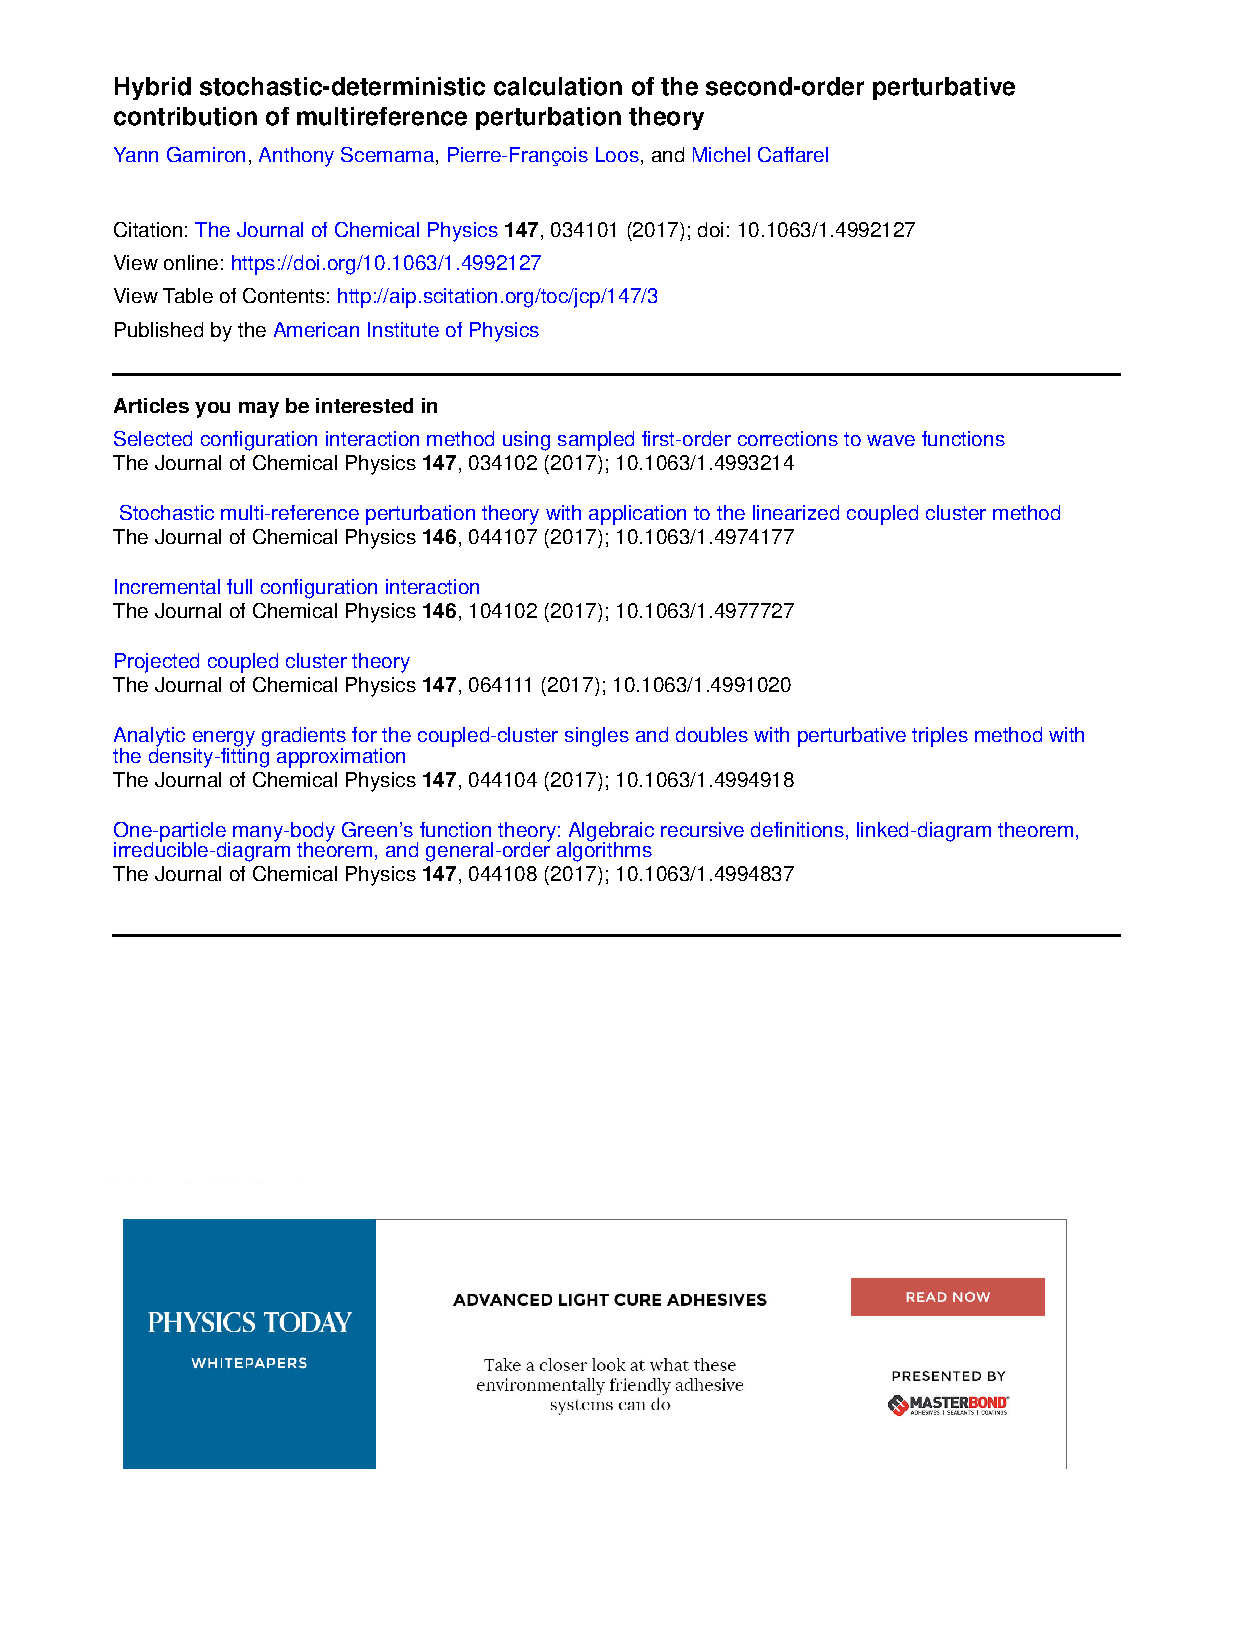
\includepdf[page=2-]{article_pt2}

\minitoc
\subfile{pt2}


\chapter{Matrix dressing}
\minitoc
\subfile{matrix_dressing}


\chapter{exponential dressing etc}
\subfile{exp_dressing}

\chapter{Performance measurements}
\subfile{perf}


\bibliographystyle{ieeetr}
\bibliography{thesis}

\appendix 

\chapter{Quantum Package basics}
\minitoc
\subfile{qp_general}

\end{document}




